\chapter{Implementacija i korisničko sučelje}
		
		
		\section{Korištene tehnologije i alati}
			Za komunikaciju između članova tima korištene su aplikacije WhatsApp\footnote{https://www.whatsapp.com/} i Microsoft Teams\footnote{https://www.microsoft.com/en-us/microsoft-teams/group-chat-software}. Upravljanje programskim kodom se obavljalo preko distribuiranog sustava Git\footnote{https://git-scm.com/} te je korišten udaljeni repozitorij GitLab\footnote{https://about.gitlab.com/}.
			
			Za izradu korisničkih sučelja, tj. frontenda, korištena je JavaScript biblioteka React ili React.js\footnote{https://reactjs.org/} koja se koristi za brzu i učinkovitu izgradnju interaktivnih korisničkih sučelja i web aplikacija uz znatno manje napisanog koda. U Reactu aplikacije se razvijaju stvaranjem komponenti za višestruku uporabu. React je izgrađen pomoću JSX-a – kombinacije JavaScripta i XML-a. Razvio ga je Facebook. Razvojna okolina korištena za rad u Reactu je Visual Studio Code\footnote{https://code.visualstudio.com/}. VS Code besplatno je Microsoftovo razvojno okruženje otvorenog koda (engl. open source). Danas jedan od najpopularnijih uređivača izvornog koda koji omogućuje programiranje u velikom izboru programskih jezika. 
			
			Implementacija ove web aplikacije, tj. backend, napravljena s radnim okvirom Spring Boot\footnote{https://spring.io/projects/spring-boot}. Spring Boot je mikro framework otvorenog koda koji održava tvrtka Pivotal. Koristi Javu te je zgrađen na temelju Spring okvira. On pruža lakši i brži način za postavljanje, konfiguriranje i pokretanje aplikacija. Za pisanje backenda korišteno je razvojno okruženje InteliJ IDEA\footnote{https://www.jetbrains.com/idea/}. To je integrirano razvojno okruženje (IDE) napisano u Javi za razvoj računalnog softvera napisanog u Javi, Kotlinu , Groovyju i drugim jezicima koji se temelje na JVM -u. Razvio ga je JetBrains. Pruža određene značajke kao što je dovršavanje koda analizom konteksta, navigacija koda koja omogućuje izravno skakanje u klasu ili deklaraciju u kodu, refaktoriranje koda , otklanjanje pogrešaka koda i opcije za ispravljanje nedosljednosti putem prijedloga.
			
			Za pisanje dokumentacije korišten je markup jezik LaTeX pisan u TeXstudio\footnote{https://www.texstudio.org/} uređivaču teksta. Za izradu dijagrama potrebnih u dokumentaciji korišteni su alati Astah Professional\footnote{https://astah.net/products/astah-professional/} i Visual Paradigm Online\footnote{https://online.visual-paradigm.com/}. Ispitivanje programskog rješenja provedeno je uz radni okvir Selenium WebDriver\footnote{https://www.selenium.dev/documentation/webdriver/}. 
			
			Za deploy frontenda korišten je Netlify\footnote{https://www.netlify.com/}, a za deploy backenda i baze podataka Render\footnote{https://render.com/}. 
			
			
			\eject 
		
	
		\section{Ispitivanje programskog rješenja}
			
			\subsection{Ispitivanje komponenti}
			
			Ispitivanje komponenti provodi se s ciljem ispitivanja pojedinih metoda i klasa, na način da se metodi daju ulazni podaci (ispravni ili neispravni) i provjerava se daje li metoda očekivani izlaz.
			
			\noindent Prilikom testiranja repository sloja koristili smo KorisnikRepository interface. Najprije smo provjerili koliko korisnika već ima u bazi kako bismo znali je li se naš novi korisnik dodao u bazu. Napravili smo novog ispravnog korisnika i pokušali ga spremiti u bazu.
			
			\begin{verbatim}
			    @Test
			    @Order(1)
			    void setData() {
			        brojKorisnika = korisnikRepositoryTest.findAll().size();
			        korisnik = new Korisnik("email@proba.com", "Test ime", 
			        "testPassword1234", false);
			        Assertions.assertNull(korisnik.getId());
			        korisnik = korisnikRepositoryTest.save(korisnik);
			    }
			\end{verbatim}
			Zatim smo provjerili postoji li jedan korisnik više u bazi i spremili njegov id kako bismo ga na kraju mogli obrisati.
			
			\begin{verbatim}
			    @Test
			    @Order(2)
			    void isSave() {
			        Assertions.assertEquals(brojKorisnika + 1,
			        korisnikRepositoryTest.findAll().size());
			        Assertions.assertNotNull(korisnik.getId());
			        idKorisnika = korisnik.getId();
			    } 
			\end{verbatim}
			Potom smo pokušali spremiti korisnika s prekratkom lozinkom što nije uspjelo, kao što je i očekivano.
			
			\begin{verbatim}
			    @Test
			    @Order(3)
		        void prekratkaLozinka() {
			        korisnik = new Korisnik("prekratkaLozinka@proba.com",
			        "Prekratka lozinka", "test12345", false);
			        Assertions.assertEquals(brojKorisnika + 1,
			        korisnikRepositoryTest.findAll().size());
			        try {
				        korisnikRepositoryTest.save(korisnik);
			        } catch (Exception e) {
				        System.out.println("Lozinka je prekratka!\n" + e);
			        }
			        Assertions.assertEquals(brojKorisnika + 1, 
			        korisnikRepositoryTest.findAll().size());
			    } 
			\end{verbatim}
			Testirali smo i slučaj kada je username prekratak. Spremanje takvog korisnika također nije uspjelo.
			
			\begin{verbatim}
			    @Test
			    @Order(4)
			    void prekratakUsername() {
			        try {
			            korisnik = new Korisnik("prekratakUsername@proba.com", 
			            "", "testLozinka12345", false);
			            Assertions.assertEquals(brojKorisnika + 1, 
			            korisnikRepositoryTest.findAll().size());
			            korisnikRepositoryTest.save(korisnik);
			        } catch (IllegalArgumentException e) {
			            System.out.println("Username je prekratak!\n" + e);
			        }
			        Assertions.assertEquals(brojKorisnika + 1,
			        korisnikRepositoryTest.findAll().size());
		    }
			\end{verbatim}
			Na kraju smo još jednom provjerili broj korisnika u bazi, te obrisali jedinog korisnika kojeg smo uspjeli uspješno spremiti.
			
			\begin{verbatim}
			    @Test
			    @Order(6)
			    void delete() {
			        Assertions.assertEquals(brojKorisnika + 1, 
			        korisnikRepositoryTest.findAll().size());
			        korisnikRepositoryTest.deleteById(idKorisnika);
			        Assertions.assertEquals(brojKorisnika, 
			        korisnikRepositoryTest.findAll().size());
			        List<Korisnik> korisnici = 
			        korisnikRepositoryTest.findAll().stream().filter(k ->
			        k.getId().equals(idKorisnika)).toList();
                    Assertions.assertEquals(0, korisnici.size());
		    }
			\end{verbatim}
			Kada pokrenemo sve testove vidimo da se oni ispravno izvode.
			
			\begin{figure}[H]
				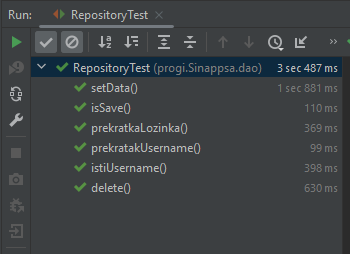
\includegraphics[scale=1]{slike/ispitivanje1.PNG} 
				\centering
				\caption{Rezultati RepositoryTest testova}
				\label{fig:RepositoryTest}
			\end{figure}
			\noindent Veoma slične testove napisali smo i za provjeru service sloja, gdje smo provjeravali KolegijService i SmjerService interface i koji također svi ispravno rade.
			
			\begin{figure}[H]
				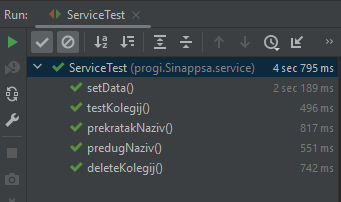
\includegraphics[scale=1]{slike/ispitivanje2.PNG} 
				\centering
				\caption{Rezultati ServiceTest testova}
				\label{fig:ServiceTest}
			\end{figure}
			
			\noindent Za provjeru controller sloja smo koristili OglasController. Na početku svakog testa zadali smo odgovarajući URL stranice, odredili vrstu HTTP zahtjeva, te postavili potrebne ulazne podatke. Za dodavanje novog oglasa najprije smo u string varijablu u JSON formatu spremili naslov, opis, idPomagaca, idKolegija i idKategorije te to postavili kao entitet zahtjeva. Nakon što se zahtjev pošalje i dobijemo odgovor provjeravamo je li se on izvršio dobro. Najprije provjeravamo je li statusLine 200, te vraća li se u odgovoru “OK” kako je i zadano u controller-u.
			
			
			\begin{verbatim}
			    @Test
			    @Order(1)
			    public void addNewOglas() throws NoSuchAlgorithmException, 
			    KeyStoreException, KeyManagementException, IOException {
			        String pageUrl ="http://localhost:8080/api/oglasi/create";
					
			        TrustStrategy acceptingTrustStrategy = (X509Certificate[] 
			        chain, String authType) -> true;
			        SSLContext sslContext = org.apache.http.ssl.SSLContexts.
			        custom().loadTrustMaterial(null, acceptingTrustStrategy)
			        .build();
			        SSLConnectionSocketFactory csf = new 
			        SSLConnectionSocketFactory(sslContext);
			        CloseableHttpClient httpClient = HttpClients.custom()
			        .setSSLSocketFactory(csf).build();
					
			        HttpPost httpPost = new HttpPost(pageUrl);
			        String JSON_STRING = "{\"naslov\":\"Oglas 
			            iz Controller testa\",\"opis\":\"Novi 
			            opis iz Controller testa\"," + "\"idPomagaca\ 
			            ":164,\"idKolegija\":140,\"idKategorije\":3}";
		            HttpEntity stringEntity = new StringEntity(JSON_STRING, 
		            ContentType.APPLICATION_JSON);
		            httpPost.setEntity(stringEntity);
					
		            CloseableHttpResponse response = httpClient.execute(httpPost);
					
		            logger.info("code={}", 
		            response.getStatusLine().getStatusCode());
		            logger.info("statusLine={}", 
		            response.getStatusLine());
		            Assertions.assertEquals(200, 
		            response.getStatusLine().getStatusCode());
		            String jsonString = 
		            EntityUtils.toString(response.getEntity());
		            logger.info("jsonString={}", jsonString);
		            Assertions.assertEquals("OK",jsonString);
			    }
			\end{verbatim}
			U ControllerTestu smo još pokušali dohvatiti sve oglase za prijavljenog korisnika kako bismo provjerili provjerava li se autorizacija na dobar način tamo gdje je ona potrebna. U header smo postavili username i password korisnika iz baze te nakon što smo dobili odgovor kojem je statusLine 200 provjeravamo počinje li odgovor sa id-om korisnika kojeg smo mu zadali.
			
			\begin{verbatim}
			    @Test
			    @Order(2)
			    public void getOglasiKorisnika() throws 
			    NoSuchAlgorithmException, KeyStoreException, 
			    KeyManagementException, IOException, JSONException {
			        //dohvati sve oglase za prijavljenog korisnika
			        String pageUrl ="http://localhost:8080/api/oglasi
			            /dohvati/korisnik";
					
			        TrustStrategy acceptingTrustStrategy = 
			        (X509Certificate[] chain, String authType) -> true;
			        SSLContext sslContext = org.apache.http.ssl
			        .SSLContexts.custom().loadTrustMaterial(null, 
			        acceptingTrustStrategy).build();
			        SSLConnectionSocketFactory csf = new 
			        SSLConnectionSocketFactory(sslContext);
		        CloseableHttpClient httpClient = HttpClients
		        .custom().setSSLSocketFactory(csf).build();
					
			        HttpGet httpGet = new HttpGet(pageUrl);
		        String auth =  username + ":" + password;
			        byte[] encodedAuth = 
			        Base64.getEncoder().encode(auth.getBytes
			        (StandardCharsets.ISO_8859_1));
			        String authHeader = "Basic " + new String(encodedAuth);
			        httpGet.setHeader(HttpHeaders.AUTHORIZATION, authHeader);
					
			        CloseableHttpResponse response = httpClient
			        .execute(httpGet);
					
		        logger.info("code={}", response.getStatusLine()
		        .getStatusCode());
			        logger.info("statusLine={}", response.getStatusLine());
			        Assertions.assertEquals(200, 
			        response.getStatusLine().getStatusCode());
			        String jsonString = EntityUtils.toString(response.getEntity());
			        logger.info("jsonString={}", jsonString);
		        Assertions.assertTrue(jsonString
		        .contains("\"id\":164,\"ime\":\"Milica\""));
			    }
			\end{verbatim}
			Controller testovi također svi rade ispravno.
			
			\begin{figure}[H]
				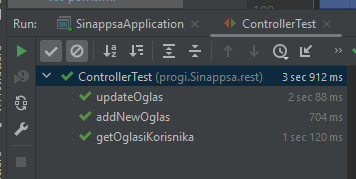
\includegraphics[scale=1]{slike/ispitivanje3.PNG} 
				\centering
				\caption{Rezultati ControllerTest testova}
				\label{fig:ControllerTest}
			\end{figure}
		
			\subsection{Ispitivanje sustava}
			
			Ispitivanje cijelog sustava napravili smo pomoću Selenium WebDrivera unutar Junit testova.
			
			\noindent Na početku imamo dva testa koja testiraju ispravnu i neispravnu prijavu. U svakom od njih naprijed definiramo postavke samo drivera, te mu zadamo URL stranice sa koje započinje test. Nakon što pronađe element u koji se upisuje username, pošaljemo mu podatke za username, te isto učinimo i za password. Budući da su podaci ispravni, aplikacija automatski preusmjerava korisnika na početnu stranicu pa se to i provjerava u posljednjem retku testa.
			
			\begin{verbatim}
			    @Test
			    public void testLogin() throws InterruptedException {
			        System.setProperty("webdriver.chrome.driver", 
			        "C:\\Program Files (x86)\\Chrome Driver\\chromedriver.exe");
			        WebDriver driver = new ChromeDriver();
			        driver.manage().timeouts().implicitlyWait(10, TimeUnit.SECONDS);
			        driver.get("https://sinappsa.netlify.app/prijava");
			        WebElement element = driver.findElement(By.name("usernameOrEmail"));
			        element.sendKeys("vmilica");
			        element = driver.findElement(By.name("password"));
			        element.sendKeys("vmilica1234");
			        driver.findElement(By.cssSelector("Button[type='submit']")).click();
			        Thread.sleep(3000);
			        String url = driver.getCurrentUrl();
			        driver.quit();
			        Assertions.assertEquals("https://sinappsa.netlify.app/", url);
		    }
			\end{verbatim}
			Test za neispravnu prijavu je skoro identičan kao za ispravnu, jedino što mu se zadaju neispravni podaci. U ovom slučaju to je neispravna lozinka i on mora na samom kraju ostati na stranici za prijavu, a ne biti preusmjeren na početnu stranicu aplikacije.
			
			\begin{verbatim}
		    @Test
		    public void failLogin() throws InterruptedException {
			        System.setProperty("webdriver.chrome.driver", 
			        "C:\\Program Files (x86)\\Chrome Driver\\chromedriver.exe");
			        WebDriver driver = new ChromeDriver();
			        driver.manage().timeouts().implicitlyWait(10, TimeUnit.SECONDS);
			        driver.get("https://sinappsa.netlify.app/prijava");
			        WebElement element = driver.findElement(By.name("usernameOrEmail"));
			        element.sendKeys("vmilica");
			        element = driver.findElement(By.name("password"));
			        element.sendKeys("vmilica123456");
			        driver.findElement(By.cssSelector("Button[type='submit']")).click();
			        Thread.sleep(3000);
			        String url = driver.getCurrentUrl();
			        driver.quit();
			        Assertions.assertEquals("https://sinappsa.netlify.app/prijava", url);
			    }
			\end{verbatim}
			Testirali smo i ponaša li se aplikacija kako treba ako se ne upišu svi potrebni podaci prilikom dodavanja novog oglasa. Naravno, za dodavanje novog oglasa korisnik mora biti prijavljen, stoga na početku testa, nakon postavki drivera slijedi prijava u aplikaciju identična prvom testu. Nakon što je prijava bila uspješna na početnoj stranici odabire se gumb “Dodaj oglas” i u tražena polja upisuju se samo naslov i opis oglasa dok smjer, kolegij i kategorija ostaju prazni što aplikacija ne bi trebala podržati. Budući da je test uhvatio iznimku, vidimo da takav oglas nije dodan u bazu podataka i zaključujemo da aplikacija radi ispravno.
			
			\begin{verbatim}
			    @Test
			    void dodavanjeOglasa() throws InterruptedException {
			        //neuspjelo
			        System.setProperty("webdriver.chrome.driver", 
			        "C:\\Program Files (x86)\\Chrome Driver\\chromedriver.exe");
			        WebDriver driver = new ChromeDriver();
			        driver.manage().timeouts().implicitlyWait(10, TimeUnit.SECONDS);
			        driver.get("https://sinappsa.netlify.app/prijava");
			        WebElement element = driver.findElement(By.name("usernameOrEmail"));
			        element.sendKeys("vmilica");
			        element = driver.findElement(By.name("password"));
			        element.sendKeys("vmilica1234");
			        driver.findElement(By.cssSelector("Button[type='submit']")).click();
			        Thread.sleep(3000);
			        String url = driver.getCurrentUrl();
			        Assertions.assertEquals("https://sinappsa.netlify.app/", url);
			        driver.findElement(By.xpath("//Button[text()='Dodaj oglas']")).click();
			        element = driver.findElement(By.name("naslov"));
			        element.sendKeys("Selenium naslov oglasa");
			        element = driver.findElement(By.name("opis"));
			        element.sendKeys("Selenium opis novog oglasa");
			        try {
			            driver.findElement(By.xpath("//Button[text()='Potvrdi']")).click();
			        } catch (Exception e) {}
			        System.out.println("Uhvatio sam iznimku!!");
			        driver.findElement(By.xpath("//button[text()='Ok']")).click();
			        Assertions.assertEquals("https://sinappsa.netlify.app/", url);
			        driver.quit();
			    }
			\end{verbatim}
			Posljednji test sustava provjerava javljanje na upite već postavljenih oglasa. Također se ni na upite ne može javljati korisnik koji nije prijavljen, stoga najprije moramo provesti valjanu prijavu. Nakon što je prijava uspjela, a to vidimo preusmjeravanjem na početnu stranicu, odabiremo oglas koji nije naš i na koji se ranije nismo javili, upisujemo poruku korisniku koji je oglas objavio i šaljemo upit.
			
			\begin{verbatim}
			    @Test
		    void dodavanjeUpita() throws InterruptedException {
			        //nije uspjelo
			        System.setProperty("webdriver.chrome.driver", 
			        "C:\\Program Files (x86)\\Chrome Driver\\chromedriver.exe");
			        WebDriver driver = new ChromeDriver();
			        driver.manage().timeouts().implicitlyWait(10, TimeUnit.SECONDS);
		            driver.get("https://sinappsa.netlify.app/prijava");
			        WebElement element = driver.findElement(By.name("usernameOrEmail"));
			        element.sendKeys("vmilica");
			        element = driver.findElement(By.name("password"));
			        element.sendKeys("vmilica1234");
			        driver.findElement(By.cssSelector("Button[type='submit']")).click();
			        Thread.sleep(3000);
			        String url = driver.getCurrentUrl();
			        Assertions.assertEquals("https://sinappsa.netlify.app/", url);
			        Thread.sleep(3000);
			        driver.findElement(By.xpath("//button[text()='Javi se']")).click();
			        element = driver.findElement(By.xpath("//textarea"));
			        element.sendKeys("Javljam se na ovaj upit iz Seleniuma!");
                    driver.findElement(By.xpath("//button[text()='Submit']")).click();
			        driver.quit();
			    }
			\end{verbatim}
			Nakon pokretanja svih testova sustava vidimo da i oni ispravno rade.
			
			\begin{figure}[H]
				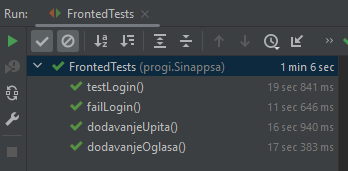
\includegraphics[scale=1]{slike/ispitivanje4.PNG} 
				\centering
				\caption{Rezultati testova sustava}
				\label{fig:FrontendTest}
			\end{figure}
			
			\eject 
		
		
		\section{Dijagram razmještaja}
			Dijagram razmještaja je strukturni statički UML dijagram koji opisuje topologiju sustava i usredotočen je na odnos sklopovskih i programskih dijelova. Na klijentskoj strani je PC računalo na kojem je pokrenut web preglednik. Klijent se protokolom HTTPS spaja na poslužitelja. Web poslužitelj i poslužitelj baze podataka nalaze se na istom računalu. Sustav je baziran na arhitekturi „klijent – poslužitelj“.
			
			\begin{figure}[H]
				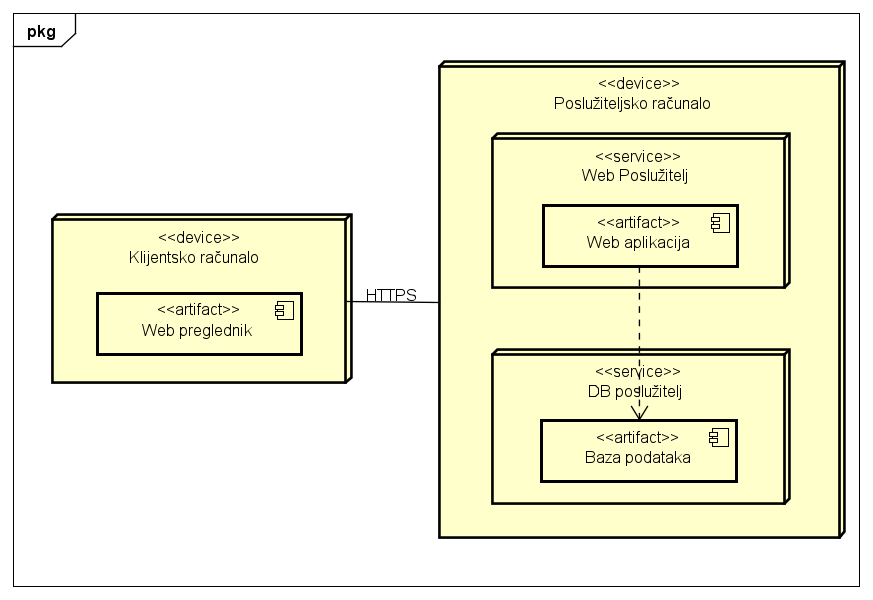
\includegraphics[scale=0.65]{dijagrami/DijagramRazmjestaja.png}
				\centering
				\caption{Dijagram razmještaja}
				\label{fig:dijagram razmjestaja}
			\end{figure}

			\eject 
		
		\section{Upute za puštanje u pogon}
			\noindent \textbf{Instalacija poslužitelja baze podataka}
			
			Na poslužitelju Render potrebno je napraviti poslužitelj baze podataka. Odabirom \textit{New} -$>$ \textit{PostgreSQL} radi se nova SQL baza. Potrebno je unijeti sljedeće podatke:
			\begin{packed_item}
				\item Ime: ime pod kojim će se baza spremati na Renderu
				\item Baza: postavljanje atributa dbname koji ćemo koristiti kod povezivanja s backend dijelom aplikacije
				\item PostgreSQL: odabir verzije PostgreSQL
			\end{packed_item}
			Opcionalno može se dodati ime korisnika (u suprotnom će se naziv korisnika slučajno generirati).
			\begin{figure}[H]
				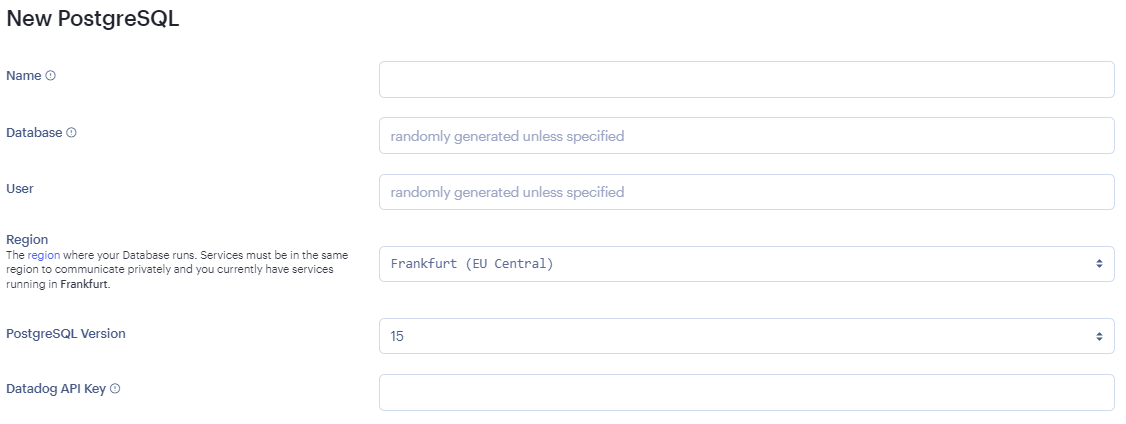
\includegraphics[scale=0.5]{slike/slika1.png}
				\centering
				\caption{Prikaz dijaloškog okvira stvaranja baze podataka}
				\label{fig:dij okvir}
			\end{figure}
			\begin{figure}[H]
				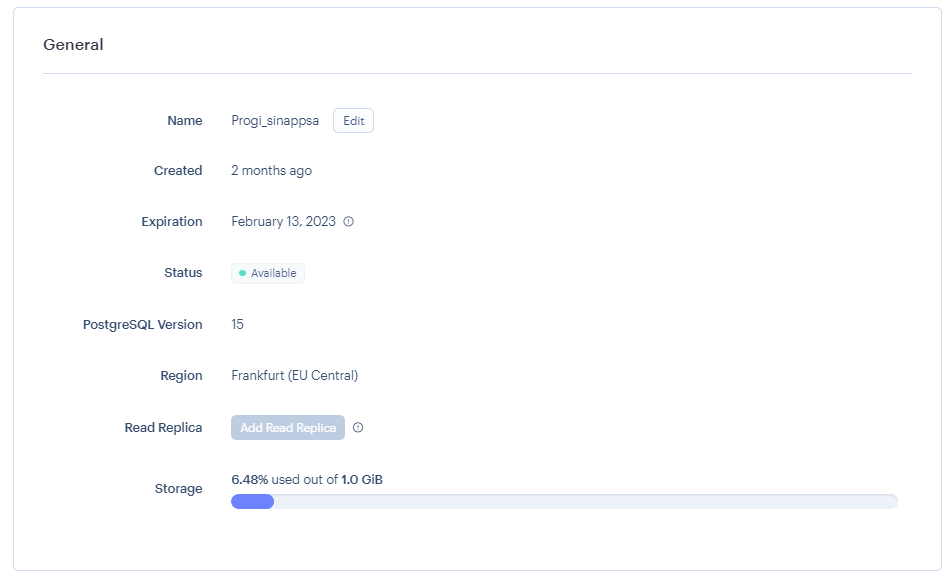
\includegraphics[scale=0.45]{slike/slika2.png}
				\centering
				\caption{Uspješno dodan poslužitelj baze podataka}
				\label{fig:uspj dodan}
			\end{figure}
			
			\noindent \textbf{Povezivanje backend dijela aplikacije s bazom podataka}
			
			U backend dijelu aplikacije, kako bismo se uspješno povezali s bazom, u Spring Boot aplikaciju u datoteku Sinappsa/src/resources/deploy/application.properties treba dodati 3 atributa:
			\begin{packed_item}
				\item spring.datasource.url 
				\item spring.datasource.username 
				\item spring.datasource.password
			\end{packed_item}
			Ove atribute treba postaviti u skladu s podacima za povezivanje na poslužitelj baze koji su dostupni na Renderu.
			\begin{figure}[H]
				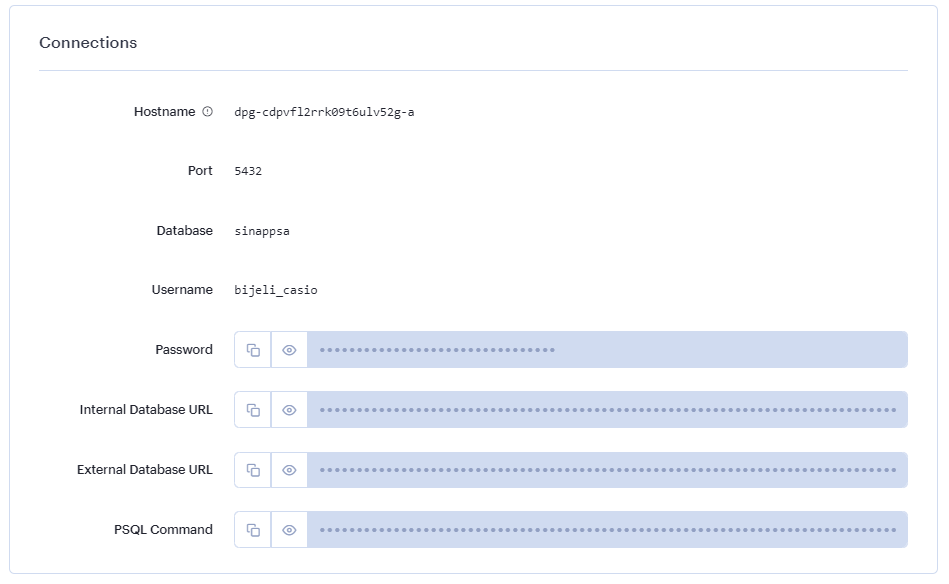
\includegraphics[scale=0.5]{slike/slika3.png}
				\centering
				\caption{Prikaz podataka potrebnih za povezivanje na poslužitelj baze podataka}
				\label{fig:povez baz pod}
			\end{figure}
			
			Atribut spring.datasource.url treba postaviti na string koji će predstavljati URL adresu poslužitelja baze podataka. Taj URL započinje sa stringom jdbc:postgresql:// te se na taj dio zalijepi \textit{Hostname} poslužitelja zajedno s portom (deafultni port je 5432) te se nakon toga doda ime baze podataka. Atribut spring.datasource.username postavlja se na \textit{Username} koji je dodijelio poslužitelj baze podataka. Atribut 
			
			\noindent spring.datasource.password poprima vrijednosti generirane zaporke koja služi za autentifikaciju pri spajanju na poslužitelj baze podataka.
			
			
			\noindent \textbf{Instalacija poslužitelja backend dijela aplikacije}
			
			Za instalaciju backend poslužitelja koristimo Render. Kako Render ne pruža podršku za Javu, prije same instalacije poslužitelja backenda potrebno je Java kod omotati u Docker izvršnu okolinu pomoću Dockerfile-a na način prikazan na slici \ref{fig:dockerfile}.
			\begin{figure}[H]
				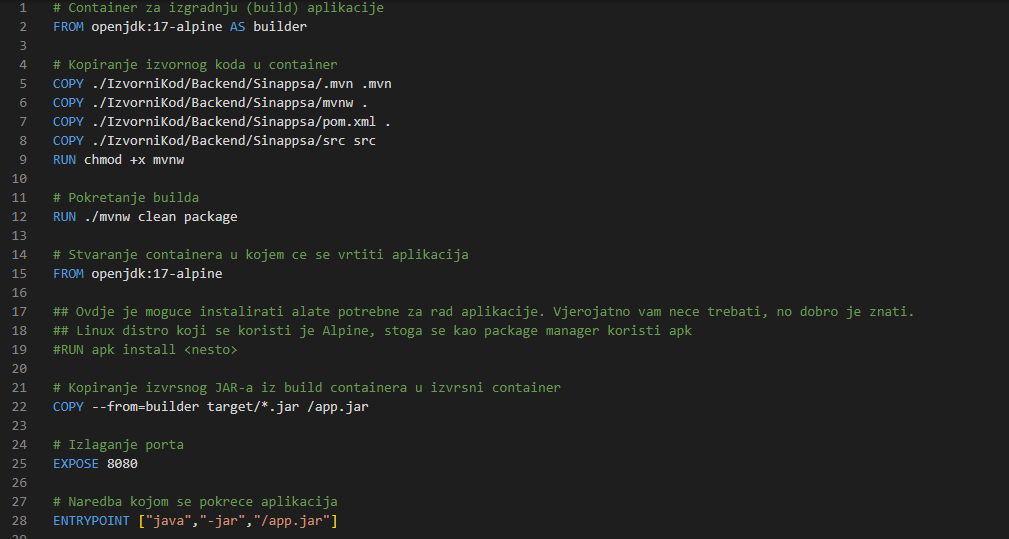
\includegraphics[scale=0.5]{slike/slika4.png}
				\centering
				\caption{Prikaz Dockerfilea}
				\label{fig:dockerfile}
			\end{figure}
			
			Kako bismo uspješno postavili poslužitelj potrebno je odabrati opciju \textit{New}-$>$\textit{Web Sevice}. Zatim se potrebno povezati sa Git repozitorijem na kojem se nalazi kod backend aplikacije. Nakon toga Render zahtjeva sljedeće parametre:
			\begin{packed_item}
				\item \textit{Name}: ime web servisa 
				\item \textit{Branch}: grana git repozitorija na kojoj se nalazi web servis 
				\item Korijenski direktorij: put do direktorija u kojem se nalazi napravljeni Dockerfile
				\item \textit{Enviroment}: odabir izvršne okoline (budući da Render nema direktnu podršku za Javu ovdje odabiremo Docker)
			\end{packed_item}
			\begin{figure}[H]
				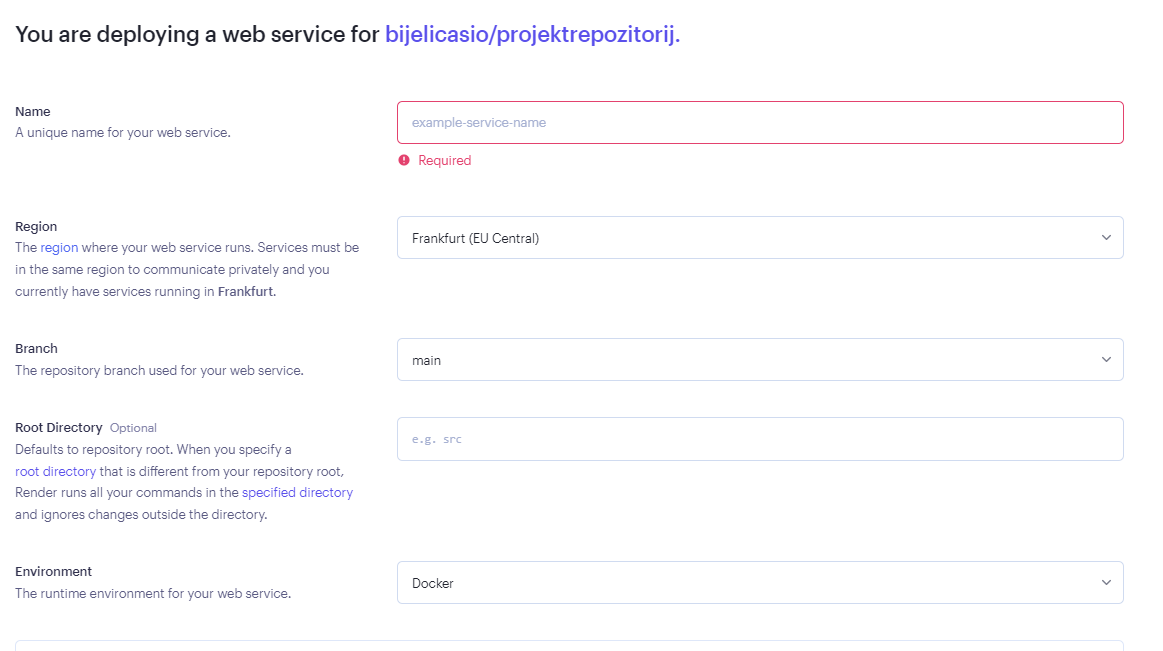
\includegraphics[scale=0.4]{slike/slika5.png}
				\centering
				\caption{Prikaz podataka potrebnih za instalaciju poslužitelja backend dijela aplikacije}
				\label{fig:backend pod}
			\end{figure}
		
			Klikom na gumb \textit{Advanced} proširuju se mogućnosti za postavljene web servisa. U \textit{Advanced} postavkama pod karticom \textit{Enviroment variables} potrebno je dodati dvije varijable izvršne okoline:
			\begin{packed_item}
				\item DB\_PASS
				\item DB\_USERNAME
			\end{packed_item}
			Ove dvije varijable postavljamo na vrijednosti \textit{usernamea} i \textit{passworda} s poslužitelja baze podataka. Odabirom opcije \textit{Create servis} započinje stvaranje servisa i stvaranje tablica u bazi podataka.
		
			
			\noindent \textbf{Pokretanje backend aplikacije i stvaranje tablica u bazi}
			
			Pokretanjem Spring Boot backend aplikacije pomoću Java Persistance API-ja koji služi za perzistenciju podataka aplikacije pomoću objektno realcijskog preslikavanja (eng. Object Relational Mapping - ORM) u povezanoj bazi podataka stvaraju se tablice iz klasa definiranih u aplikaciji koje su anotirane oznakom \textit{@Entity}. 
			
			Uspješnim deployom backend aplikacije ona postaje dostupna za rad preko interneta. Pomoću kartice \textit{Logs} na Renderu moguće je pratiti zahtjeve koji pristižu na servis te odgovore na zahtjeve i eventualne greške.
			
			
			\noindent \textbf{Instalacija poslužitelja frontenda}
			
			Za pogon frontend dijela aplikacije ne koristimo Render, već Netlify. Nakon uspješnog stvaranja tima na Netlifyu odabirom opcije \textit{Add new Site} pod kategorijom \textit{Site} možemo deployati stranicu. Nakon \textit{Add new Site} odabiremo opciju \textit{Import an existing project} te se povezemo sa Git repozitorijem. Nakon odabira repozitorija odabiremo granu u repozitoriju na kojem se nalazi izvorni kod dijela stranice i u polje \textit{Base directory} stavljamo putanju do mape u kojoj se nalazi izvorni kod. Za \textit{build command} postavljamo naredbu \textit{npm run build}. 
			\begin{figure}[H]
				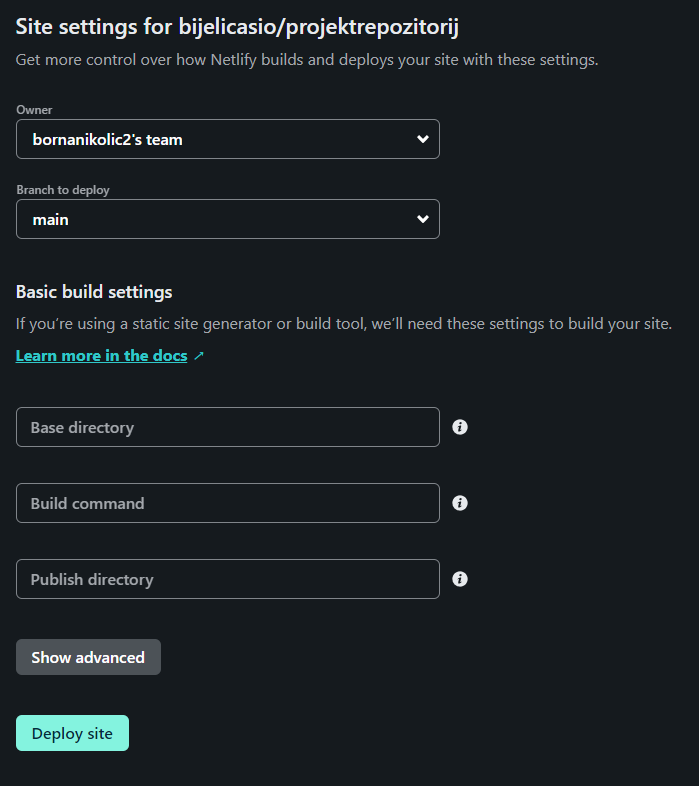
\includegraphics[scale=0.5]{slike/slika6.png}
				\centering
				\caption{Prikaz podataka potrebnih za instalaciju frontend poslužitelja}
				\label{fig:frontend pod}
			\end{figure}
			
			Odabirom opcije \textit{Deploy site} kreće se u \textit{build frontend} i po uspješnom završetku web aplikacija je puštena u pogon na javnom poslužitelju.
			\eject 